\documentclass{iopjournal}

\usepackage{amsmath,amssymb,amsfonts}
\usepackage{amsthm}

\theoremstyle{plain}
\newtheorem{theorem}{Theorem}
\newtheorem{proposition}[theorem]{Proposition}
\newtheorem{corollary}[theorem]{Corollary}
\newtheorem{lemma}[theorem]{Lemma}
\theoremstyle{remark}
\newtheorem{remark}[theorem]{Remark}

\newcommand{\dd}{\mathrm{d}}

\begin{document}
\fancyhead[R]{D Janzen\ }

\articletype{Paper}

\title{The Schwarzschild horizon and singularity as the two poles of one circle: the analytic structure of the maximally extended geometry}

\author{Daryl Janzen}

\affil{Department of Physics and Engineering Physics, University of Saskatchewan, 116 Science Place, Saskatoon, SK S7N 5E2, Canada}

\email{daryl.janzen@usask.ca}

\keywords{Schwarzschild geometry, maximal extension, singularity classification, analytic continuation, Kretschmann scalar}

\begin{abstract}
The standard account of the Schwarzschild geometry treats its event horizon and its central singularity as objects of different kinds: the first a removable coordinate singularity, the second a curvature singularity at which the spacetime ends. Both judgements are correct as statements about extending the Lorentzian manifold. We ask whether the analytic structure of the geometry draws the same distinction, and find that it does not. In Lemaître--Tolman cycloid coordinates the areal radius is $r(z)=M(1+\cos z)$, and the horizon and $r=0$ are its two non-degenerate critical points, of identical analytic character: the two poles of the circle $(r-M)^2+(\dd r/\dd z)^2=M^2$. Continuing $z$ into the complex plane by the same operation at each pole gives one analytic curve whose real sections are the four regions of the Kruskal--Szekeres extension and, beyond $r=0$, two regions at $r<0$ isometric to Schwarzschild of negative mass; we prove these are the only real sections. The asymmetry of the standard classification is located exactly: the two poles are indistinguishable through first order and separated at second order by the single value the areal radius takes at each, $2M$ against $0$, which the Kretschmann scalar reads through a twelfth-order pole. The approach to $r=0$ is universal: along every radial timelike geodesic the curvature tends to $64/27s^4$ in the proper time $s$ remaining, independent of mass and energy. The two loci are critical points of one curve, differing in one number. The spacetime's inextendibility results are untouched.
\end{abstract}

\section{Introduction}\label{sec:intro}

The maximal analytic extension of the Schwarzschild solution, formulated by Synge~\cite{synge1950} and developed by Kruskal~\cite{kruskal1960} and Szekeres~\cite{szekeres1960}, consists of four regions joined at a bifurcation 2-sphere: two asymptotically flat exteriors and two interiors, each interior bounded by a spacelike curvature singularity at $r=0$. The standard account classifies the two distinguished loci of this geometry as objects of different kinds. The horizon at $r=2M$ is a coordinate singularity of the Schwarzschild chart, removed by charts---Kruskal--Szekeres, Eddington--Finkelstein, Lemaître---in which the metric extends smoothly across it. The locus $r=0$ is a scalar curvature singularity in the classification of Ellis and Schmidt~\cite{EllisSchmidt1977}: the Kretschmann scalar $K=R_{abcd}R^{abcd}=48M^{2}/r^{6}$ diverges along every incomplete geodesic that reaches it, so no extension of the spacetime with a twice-differentiable metric can contain the points those geodesics approach~\cite{Hawking1973,Wald1984}, and Sbierski has shown that no extension exists even with a merely continuous metric~\cite{sbierski2018}.

Both judgements are correct, and nothing in this paper disputes either. They are statements about the Lorentzian manifold: whether its metric admits an extension across a locus, and of what regularity. This paper asks a different question. Does the \emph{analytic} structure of the geometry---the dependence of the areal radius on a natural parameter along the radial direction, and the continuation of that dependence---distinguish the two loci in the same way? The answer is no, and the way it fails to is precise enough to say exactly where the distinction the standard account draws comes from.

The vehicle is the cycloid parametrisation of the interior, due to Lemaître and Tolman~\cite{lemaitre1933,Tolman1934} and used by Bondi~\cite{Bondi1947}, in which the areal radius is
\begin{equation}\label{eq:cycloid}
r(z)=M(1+\cos z),\qquad z\in[0,\pi],
\end{equation}
running from the horizon $r=2M$ at $z=0$ to $r=0$ at $z=\pi$. We establish five things.

\begin{enumerate}
\item The horizon and $r=0$ are the two critical points of $r(z)$, both non-degenerate, with $\dd r/\dd z=0$ and $\dd^{2}r/\dd z^{2}=\mp M$. They are the two poles of the circle $(r-M)^2+(\dd r/\dd z)^2=M^2$, which has no distinguished point (section~\ref{sec:critical}).
\item Continuing $z$ into the complex plane by the same operation at each pole gives a single analytic curve. Its real sections at $r\geq0$ are the four Kruskal--Szekeres regions; beyond $r=0$ the same operation that reaches the exterior from the interior reaches two regions at $r<0$, isometric to Schwarzschild of negative mass (section~\ref{sec:continuation}).
\item These are the only real sections: exactly three directions in the complex $z$-plane keep the areal radius real, and the two beyond the real axis are counted by the two fixed points of the reflection $z\mapsto-z$, which are the horizon and $r=0$ (Proposition~\ref{prop:exhaustive}).
\item The difference between the two poles is located exactly. They are indistinguishable through first order in derivatives of the metric. At second order the curvature separates them, and it does so through one number, the value the areal radius takes at the critical point. The Kretschmann scalar reads that value through a pole of order $12=2\times6$ at $r=0$ (section~\ref{sec:asymmetry}).
\item The approach to $r=0$ carries no trace of the collapsing body: along every radial timelike geodesic $K\to64/27s^{4}$ in the proper time $s$ remaining, independent of the mass and of the energy (Proposition~\ref{prop:universal}).
\end{enumerate}

The paper does not remove the curvature singularity at $r=0$, and does not claim the spacetime extends through it. What it shows is that the analytic structure treats the two loci as the same kind of object---two critical points of one curve---and that the whole of what the standard account reads as a difference in kind is carried by the value of the areal radius at each. section~\ref{sec:extendibility} states precisely what this does and does not imply about extendibility, and section~\ref{sec:reading} sets out the interpretive question it leaves.

\section{The cycloid parametrisation of the interior}\label{sec:cycloid}

The Schwarzschild line element in standard coordinates is, in units $G=c=1$,
\begin{equation}
ds^{2}=-\Bigl(1-\frac{2M}{r}\Bigr)dt^{2}+\Bigl(1-\frac{2M}{r}\Bigr)^{-1}dr^{2}+r^{2}d\Omega^{2},
\end{equation}
with $d\Omega^{2}$ the metric of the unit 2-sphere. For $r<2M$ the coordinates $t$ and $r$ exchange roles and $r$ is timelike.

\begin{proposition}[Lemaître--Tolman cycloid]\label{prop:cycloid}
In the interior $0<r<2M$, the radial timelike geodesic of zero Killing energy, $(\dd r/\dd\tau)^{2}=2M/r-1$, which has $\dd r/\dd\tau=0$ at $r=2M$, is
\begin{equation}\label{eq:cycloid_pair}
r(\eta)=M(1+\cos\eta),\qquad \tau(\eta)=M(\eta+\sin\eta),\qquad \eta\in[0,\pi],
\end{equation}
with $\eta=0$ at the horizon and $\eta=\pi$ at $r=0$. The proper time from horizon to $r=0$ is $M\pi$.
\end{proposition}

\begin{proof}
On the geodesic, $\dd\tau^{2}=r\,\dd r^{2}/(2M-r)$. With $r=M(1+\cos\eta)=2M\cos^{2}(\eta/2)$, $2M-r=2M\sin^{2}(\eta/2)$ and $\dd r=-M\sin\eta\,\dd\eta$, this gives $\dd\tau^{2}=4M^{2}\cos^{4}(\eta/2)\,\dd\eta^{2}$, so $\dd\tau=M(1+\cos\eta)\,\dd\eta$ and $\tau=M(\eta+\sin\eta)$ with $\tau(0)=0$.
\end{proof}

\begin{remark}
The pair~\eqref{eq:cycloid_pair} is a cycloid, the curve traced by a point on a circle of radius $M$ rolling along a line. It is also, under $M\leftrightarrow a_{m}/2$, the scale factor and cosmic time of the closed dust Friedmann--Lemaître universe, $a(\eta)=\tfrac{a_{m}}{2}(1+\cos\eta)$ and $t(\eta)=\tfrac{a_{m}}{2}(\eta+\sin\eta)$. This is the content of Oppenheimer--Snyder collapse~\cite{Oppenheimer1939b}, in which a homogeneous dust ball's interior is a portion of a closed Friedmann universe, read here at the level of the vacuum areal radius.
\end{remark}

\begin{lemma}[The interior metric]\label{lem:interior_metric}
In coordinates $(\eta,t,\theta,\phi)$ the Schwarzschild interior metric is
\begin{equation}\label{eq:interior_metric}
ds^{2}_{\mathrm{int}}=-4M^{2}\cos^{4}(\eta/2)\,\dd\eta^{2}+\tan^{2}(\eta/2)\,\dd t^{2}+M^{2}(1+\cos\eta)^{2}\,d\Omega^{2}.
\end{equation}
\end{lemma}

\begin{proof}
In the interior $g_{tt}=2M/r-1=\tan^{2}(\eta/2)$ and $g_{rr}\,\dd r^{2}=-r\,\dd r^{2}/(2M-r)=-4M^{2}\cos^{4}(\eta/2)\,\dd\eta^{2}$ by the computation in Proposition~\ref{prop:cycloid}; the angular coefficient is $r^{2}$.
\end{proof}

\section{The two critical points}\label{sec:critical}

Extend the parameter to $z\in\mathbb{R}$ and regard $r(z)=M(1+\cos z)$ as a smooth $2\pi$-periodic function, that is, a function on the circle $\mathbb{R}/2\pi\mathbb{Z}$.

\begin{proposition}[Symmetric critical points]\label{prop:critical}
The critical points of $r(z)$ are $z\in\pi\mathbb{Z}$, and all are non-degenerate. At $z=2k\pi$, $r=2M$ and $\dd^{2}r/\dd z^{2}=-M$; at $z=(2k+1)\pi$, $r=0$ and $\dd^{2}r/\dd z^{2}=+M$.
\end{proposition}

\begin{proof}
$\dd r/\dd z=-M\sin z$ vanishes exactly on $\pi\mathbb{Z}$, and $\dd^{2}r/\dd z^{2}=-M\cos z=\mp M\neq0$ there; non-degeneracy is Morse's condition~\cite{Milnor1963}.
\end{proof}

The identity of the two critical points is not a property of the particular function chosen; it is forced by the arc. Since $r-M=M\cos z$ obeys $r''=-(r-M)$, the interior arc is the projection onto the $r$-axis of uniform motion on the circle
\begin{equation}\label{eq:circle}
(r-M)^{2}+s^{2}=M^{2},\qquad s=\frac{\dd r}{\dd z},
\end{equation}
which is also the phase-space orbit of the harmonic oscillator $r''=-(r-M)$ at fixed energy. The horizon and $r=0$ are the two points at which this circle meets the $r$-axis: its two poles, the two ends of the diameter $[0,2M]$. At a pole the tangent is orthogonal to the axis, so $\dd r/\dd z=0$ there of necessity; the circle has no distinguished point, so its two poles are exchanged by the reflection through its centre; and the reflection $z\mapsto-z$, under which $r$ is even, fixes exactly the two of them. The only feature that tells the poles apart is extrinsic to the circle: the value of the areal radius at each, $2M$ at one and $0$ at the other.

\section{Continuation through both critical points}\label{sec:continuation}

The interior arc admits analytic continuation through each of its endpoints, and the same operation does it at both.

\subsection{At $z=0$: the exteriors}

\begin{proposition}\label{prop:exterior}
Under $z=i\rho$, $\rho>0$, the areal radius becomes $r=M(1+\cosh\rho)\in(2M,\infty)$ and the metric~\eqref{eq:interior_metric} becomes
\begin{equation}\label{eq:exterior}
ds^{2}=-\tanh^{2}(\rho/2)\,\dd t^{2}+4M^{2}\cosh^{4}(\rho/2)\,\dd\rho^{2}+M^{2}(1+\cosh\rho)^{2}\,d\Omega^{2},
\end{equation}
the Schwarzschild exterior in the radial coordinate $\rho$.
\end{proposition}

\begin{proof}
With $\dd z^{2}=-\dd\rho^{2}$, $\cos(i\rho/2)=\cosh(\rho/2)$ and $\tan(i\rho/2)=i\tanh(\rho/2)$, the coefficients of~\eqref{eq:interior_metric} become those of~\eqref{eq:exterior}. With $r=2M\cosh^{2}(\rho/2)$ one has $1-2M/r=\tanh^{2}(\rho/2)$ and $\dd r^{2}/(1-2M/r)=4M^{2}\cosh^{4}(\rho/2)\,\dd\rho^{2}$, which is the Schwarzschild exterior.
\end{proof}

The continuation turns the circular functions of the interior into the hyperbolic functions of the exterior, and with them the timelike parameter into a spacelike one. The conjugate branch $z=-i\rho$ gives the same $r$, since $\cosh$ is even, and so a second exterior isometric to the first; the two meet at the bifurcation sphere $r=2M$.

\subsection{At $z=\pi$: the regions at $r<0$}

\begin{proposition}\label{prop:negative}
Under $z=\pi+i\rho'$, $\rho'>0$, the areal radius becomes $r=M(1-\cosh\rho')\in(-\infty,0)$ and the metric~\eqref{eq:interior_metric} becomes
\begin{equation}\label{eq:negative}
ds^{2}=-\coth^{2}(\rho'/2)\,\dd t^{2}+4M^{2}\sinh^{4}(\rho'/2)\,\dd\rho'^{2}+M^{2}(1-\cosh\rho')^{2}\,d\Omega^{2},
\end{equation}
which is the Schwarzschild metric at $r<0$, with $1-2M/r=\coth^{2}(\rho'/2)>1$.
\end{proposition}

\begin{proof}
With $\dd z^{2}=-\dd\rho'^{2}$, $\cos((\pi+i\rho')/2)=-i\sinh(\rho'/2)$ and $\tan((\pi+i\rho')/2)=i\coth(\rho'/2)$, the coefficients become those of~\eqref{eq:negative}. With $r=M(1-\cosh\rho')=-2M\sinh^{2}(\rho'/2)$ one has $1-2M/r=(1+\cosh\rho')/(\cosh\rho'-1)=\coth^{2}(\rho'/2)$, and $\dd r^{2}/(1-2M/r)=4M^{2}\sinh^{4}(\rho'/2)\,\dd\rho'^{2}$.
\end{proof}

Since $1-2M/r>1$ throughout, these regions are static, contain no horizon, and are asymptotically flat as $r\to-\infty$. Writing $r=-\tilde r$ with $\tilde r>0$ gives $1-2M/r=1+2M/\tilde r$, the Schwarzschild metric of mass $-M$ in the areal coordinate $\tilde r$: the regions at $r<0$ are isometric to negative-mass Schwarzschild, with its naked timelike singularity at $\tilde r=0$~\cite{Bondi1957}. The conjugate branch $z=\pi-i\rho'$ gives a second such region.

\begin{remark}
Regions of negative areal coordinate are a familiar part of the maximally extended Kerr geometry, where Carter's extension continues through the disk bounded by the ring singularity into an asymptotically flat region at $r<0$ that behaves as a spacetime of negative mass~\cite{Carter1968}; whether that gluing is analytic has been questioned~\cite{GarciaCompeanManko2012}. In Schwarzschild the Kruskal--Szekeres extension restricts $r$ to non-negative values. What the cycloid adds is not the existence of a negative-mass region but its place: it is reached from the same interior arc, by the same continuation that reaches the exterior, at the other critical point.
\end{remark}

\subsection{The single curve, and why it has exactly three real directions}

\begin{proposition}[The completed curve]\label{prop:curve}
The analytic completion of the interior arc is a single curve---hyperbola, circle, hyperbola---with non-degenerate critical points at $z=0$ ($r=2M$) and $z=\pi$ ($r=0$). The Schwarzschild $(t,r)$ chart, whose coordinates degenerate at both critical points, draws it as six regions:
\begin{enumerate}
\item the black-hole interior, $z=\eta\in(0,\pi)$, and the white-hole interior, $z=\eta\in(-\pi,0)$, both with $r\in(0,2M)$;
\item two exteriors, $z=\pm i\rho$, with $r\in(2M,\infty)$, meeting at the bifurcation sphere;
\item two regions at $r<0$, $z=\pi\pm i\rho'$, horizonless and asymptotically flat.
\end{enumerate}
The four regions at $r\geq0$ are the maximal Kruskal--Szekeres extension; the two at $r<0$ lie beyond it.
\end{proposition}

\begin{proof}
The interiors are Lemma~\ref{lem:interior_metric}, the white-hole arc following because~\eqref{eq:interior_metric} is even in $\eta$; the exteriors are Proposition~\ref{prop:exterior} with both branches; the regions at $r<0$ are Proposition~\ref{prop:negative} with both branches. The four regions at $r\geq0$ join at the bifurcation sphere in the Kruskal--Szekeres arrangement and terminate at $r=0$.
\end{proof}

\begin{proposition}[Exactly three real directions]\label{prop:exhaustive}
Writing $z=a+ib$, the areal radius is real if and only if $b=0$ or $a\in\pi\mathbb{Z}$. Up to the period, the continuation therefore has exactly three real directions: the real axis (the interiors), $a=0$ (the exteriors) and $a=\pi$ (the regions at $r<0$). On them the proper-time function $\tau(z)=M(z+\sin z)$ is respectively real, imaginary, and $M\pi$ plus an imaginary number, and the three ranges $0\leq r\leq2M$, $r\geq2M$ and $r\leq0$ partition the real line.
\end{proposition}

\begin{proof}
$\cos(a+ib)=\cos a\cosh b-i\sin a\sinh b$, so $\operatorname{Im}r=-M\sin a\sinh b$, a product vanishing exactly when $b=0$ or $\sin a=0$. The values of $\tau$ follow from $\sin(ib)=i\sinh b$ and $\sin(\pi+ib)=-i\sinh b$.
\end{proof}

The two directions beyond the real axis are not placed arbitrarily. They leave the real axis at the fixed points of the reflection $z\mapsto-z$, under which $r$ is even and $\tau$ odd, and those fixed points are $z=0$ and $z=\pi$: the horizon and $r=0$. The number of continuations beyond the interior is the number of poles of the circle. A generic complex value of $z$ gives a complex areal radius and so no region of the real geometry; the real geometry is exhausted by the three directions of Proposition~\ref{prop:exhaustive}.

\begin{figure}[t]
\centering
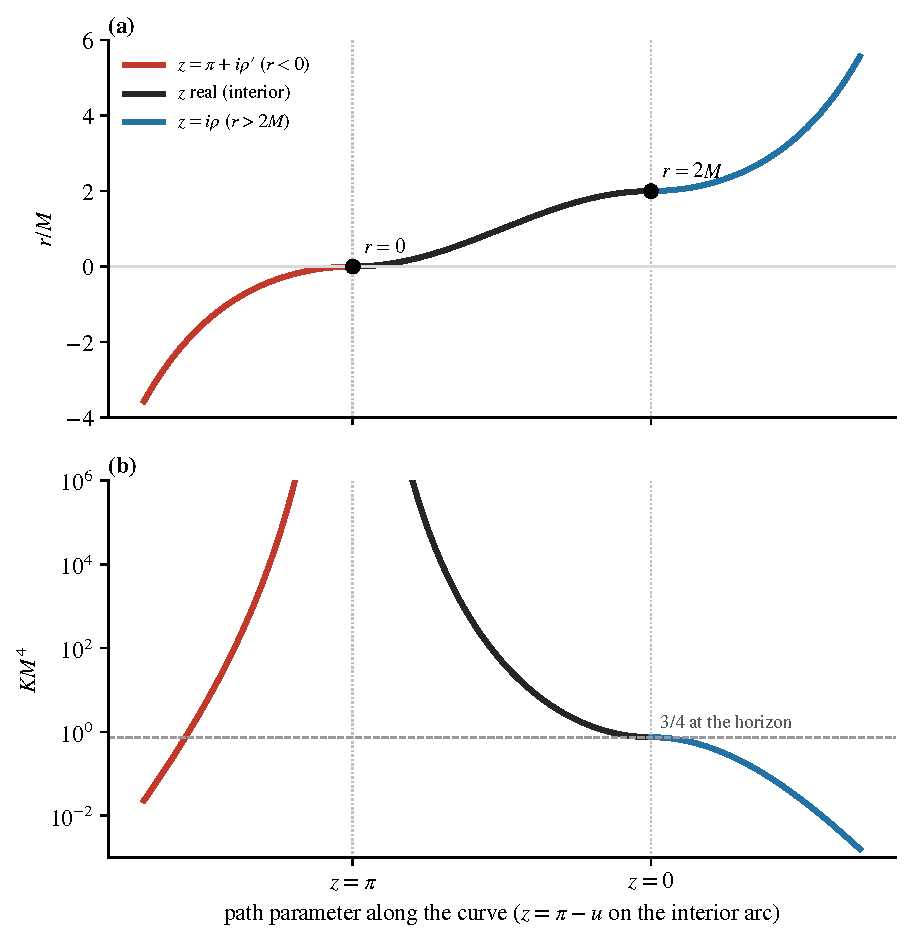
\includegraphics[width=0.7\textwidth]{fig_circle.pdf}
\caption{The completed curve. \textbf{(a)} The areal radius along the three real directions of Proposition~\ref{prop:exhaustive}: the regions at $r<0$ (red, $z=\pi+i\rho'$), the interior arc (black, $z$ real) and the exterior (blue, $z=i\rho$), in units of $M$. Both critical points have a horizontal tangent, $\dd r/\dd z=0$, and nothing in the curve distinguishes one from the other. \textbf{(b)} The Kretschmann scalar $K=48M^{2}/r^{6}$ along the same curve, in units of $M^{-4}$. It is finite, $3/4M^{4}$, at the critical point where $r=2M$ and diverges at the critical point where $r=0$, from both sides.}
\label{fig:circle}
\end{figure}

\section{Where the asymmetry lives}\label{sec:asymmetry}

The standard account distinguishes the horizon from $r=0$. The analytic structure does not. The question is then where the distinction enters, and it can be answered by the order in derivatives of the metric at which it first appears.

At zeroth order there is nothing to separate: each locus is a critical point of the areal radius, and the Schwarzschild chart degenerates at both. At first order there is still nothing. No scalar invariant of a metric is built from its first derivatives alone, the connection being removable at a point by a choice of coordinates, so no first-order quantity can register a difference between two points. The first scalar invariants are second order, the curvature invariants, and they do separate the two loci. For the Schwarzschild geometry every curvature invariant is a function of the areal radius alone, so what they separate the loci by is one number: the value of $r$ at the critical point.

\begin{proposition}[The Kretschmann pole]\label{prop:kretschmann}
As a function of $z$, the Kretschmann scalar
\begin{equation}
K(z)=\frac{48M^{2}}{r(z)^{6}}=\frac{48}{M^{4}(1+\cos z)^{6}}
\end{equation}
is finite at $z=0$, where $K=3/4M^{4}$, and has a pole of order twelve at $z=\pi$, $K=3072/(M^{4}\epsilon^{12})+O(\epsilon^{-10})$ with $\epsilon=\pi-z$. The order is the product of the order to which $r(z)$ vanishes at the critical point, two, and the power of $r$ in $K$, six.
\end{proposition}

\begin{proof}
Near $z=\pi$, $1+\cos z=1-\cos\epsilon=\epsilon^{2}/2+O(\epsilon^{4})$, so $(1+\cos z)^{6}=\epsilon^{12}/64\,(1+O(\epsilon^{2}))$ and $K=3072/(M^{4}\epsilon^{12})+O(\epsilon^{-10})$.
\end{proof}

Both critical points are non-degenerate, so $r-r_{*}$ vanishes to second order at each. What makes the pole appear at one and not the other is the value $r_{*}$: a function of $r$ singular at $r=0$, composed with a curve that reaches $r=0$ at a critical point, acquires a pole whose order is fixed by the chain rule. The Kretschmann scalar is a genuine invariant of the Schwarzschild metric and its divergence is a genuine property of that metric. What the cycloid adds is the exact location of the source of the divergence. It is not a feature of the analytic structure, which is the same at both poles; it is the value the areal radius takes at one of them.

The same holds of every other way the two loci differ in the full metric. At the horizon $g_{tt}=\tan^{2}(\eta/2)\to0$ while the 2-sphere keeps its area $16\pi M^{2}$; at $r=0$ the 2-sphere's area goes to zero while $g_{tt}\to\infty$. Each of these is a function of the value of $r$ at the critical point, and the opposition between them is the one difference, read in different components.

\begin{proposition}[The approach to $r=0$ is universal]\label{prop:universal}
Along every radial timelike geodesic reaching $r=0$, with $s$ the proper time remaining,
\begin{equation}
K\,s^{4}\longrightarrow\frac{64}{27}\qquad(s\to0),
\end{equation}
independently of $M$ and of the geodesic's energy. On the marginally bound geodesic the relation is exact at every $s$, $K=64/27s^{4}$, and the radial tidal eigenvalue $-2M/r^{3}$ equals $-4/9s^{2}$ exactly.
\end{proposition}

\begin{proof}
A radial timelike geodesic of energy $E$ obeys $(\dd r/\dd s)^{2}=E^{2}-1+2M/r$. As $r\to0$ the last term dominates, so $r\simeq(9M/2)^{1/3}s^{2/3}$, and $K=48M^{2}/r^{6}\simeq48M^{2}/((9M/2)^{2}s^{4})=64/27s^{4}$. For the marginally bound geodesic, $E=1$, the approximation is the equation itself, so the relations hold exactly. On the cycloid, $E=0$, one finds $s=M\epsilon^{3}/6+O(\epsilon^{5})$ with $\epsilon=\pi-z$, and Proposition~\ref{prop:kretschmann} gives the same limit.
\end{proof}

The mass cancels because the amplitude of $r(s)$ scales as $M^{1/3}$ and $K$ as $M^{2}/r^{6}$: $6\times\tfrac13=2$. The final approach to $r=0$ therefore carries no information about the body whose collapse produced it: every infall, whatever its mass or energy, ends along the same curvature history. The history is a known one: near $r=0$ the interior takes the form of the vacuum Kasner metric with exponents $(-\tfrac13,\tfrac23,\tfrac23)$~\cite{Kasner1921}, whose Kretschmann scalar is $-16p_{1}p_{2}p_{3}/s^{4}=64/27s^{4}$. The areal radius follows the matter-dominated law $r\propto s^{2/3}$ along the way, but the curvature is pure Weyl curvature, and not a dust universe's $80/27s^{4}$. The contrast with the horizon is exact. There $K=3/4M^{4}$ is finite and depends on the mass; at $r=0$ the divergence is universal.

\section{What this does and does not show about extendibility}\label{sec:extendibility}

The continuation of section~\ref{sec:continuation} is a continuation of the curve: of the areal radius $r(z)$ and of the metric coefficients as analytic functions of $z$. It is not an extension of the Lorentzian manifold across $r=0$. At $z=\pi$ the metric~\eqref{eq:interior_metric} degenerates, its angular part vanishing and $g_{tt}$ diverging, so it defines no Lorentzian metric in a neighbourhood of that point, and the regions at $r<0$ are not attached to the interior by any metric extension. The results on the spacetime stand as stated: the divergence of $K$ along incomplete geodesics rules out any $C^{2}$ extension containing their endpoints~\cite{Hawking1973,Wald1984}, and Sbierski's theorem rules out any $C^{0}$ extension at all~\cite{sbierski2018}. Infalling worldlines end at $r=0$ at finite proper time, $M\pi$ after crossing the horizon on the cycloid.

What the construction does bear on is the reading of the standard classification. That classification is often stated as a difference in kind: the horizon an artefact of a bad chart, an ordinary place that a good chart reveals; $r=0$ an edge at which the description itself must stop. Neither half is a statement the analytic structure makes. It does not single out the horizon as an ordinary place: the horizon is a critical point of the same kind as $r=0$, and the Schwarzschild chart degenerates at both; at the horizon this appears in the present coordinates as $g_{tt}=\tan^{2}(\eta/2)\to0$ at $z=0$. And $r=0$ is not an edge of the analytic description: the curve has no endpoint there, and continues through it by the same operation that carries it through the horizon. What separates the two is real and invariant---the curvature, finite at one and divergent at the other---and it is carried entirely by the value of the areal radius at the critical point. Both regularity statements about the spacetime are true. Reading them as a difference in what the two loci \emph{are}, rather than in the value of one function at two points of the same kind, is what the analytic structure does not support.

The two loci are drawn alike by the Schwarzschild chart, each spread into an extended line by coordinates that degenerate there, and the resemblance invites the comparison with a map projection's pole: a single point drawn as a line because the coordinate parametrising its approach is undefined at it. For the horizon the comparison is the familiar one: the line at $r=2M$ in an Eddington--Finkelstein diagram is a single place drawn out along the coordinate $v$, where $g_{tt}$ and with it the separation in $t$ vanish. At $r=0$ the drawn line is the spacelike locus along which $g_{tt}$, and with it the separation in $t$, diverges, while the collapse is in the orthogonal 2-sphere, whose area vanishes. In both cases the Schwarzschild chart draws a place as a line, by a coordinate that degenerates at a critical point of the areal radius; the degeneracies are opposite, and which one occurs is set by the value of $r$ at the critical point.

\section{The interpretive question the construction leaves}\label{sec:reading}

Two readings of the construction are available, and the analysis above does not choose between them. On the standard reading the Lorentzian manifold is the fundamental object, the cycloid parameter is a convenient coordinate on part of it, and the curvature divergence at $r=0$ is a property of the geometry. On the alternative reading the analytic curve is the more basic object and the areal radius is a function on it, so that the Schwarzschild chart is a projection of the curve by that function; the divergence is then a property of the projection, real as such, generated where the projection takes the value zero at a critical point. The two readings agree on every observable in the region $r\geq2M$, and on every statement made in sections~\ref{sec:cycloid}--\ref{sec:extendibility}. They differ on whether the difference located in section~\ref{sec:asymmetry} belongs to the geometry or to the projection.

What would decide between them is a geometric structure on which the curve is natural and from which the Schwarzschild metric is derived rather than assumed; the cycloid alone does not supply one. The alternative reading has one explanatory advantage the standard reading lacks: it accounts for why two analytically identical critical points are charted asymmetrically, by the values the projecting function takes at them, where the standard reading takes the asymmetry as given. We record that advantage and do not rest anything on it.

One further fact belongs with the construction. The single horizon of Schwarzschild is a feature of $\Lambda=0$. With a positive cosmological constant the structure function is $f=1-2M/r-r^{2}/\alpha^{2}$, $\alpha=\sqrt{3/\Lambda}$, and the horizon condition $r^{3}-\alpha^{2}r+2M\alpha^{2}=0$ is a cubic, which for $0<27M^{2}<\alpha^{2}$ has three real roots summing to zero: the black-hole and cosmological horizons, and one negative root. As $\alpha\to\infty$ the cubic degenerates to $r=2M$ and the other two roots leave to infinity. The statement that the regions at $r<0$ contain no horizon is therefore a statement about $\Lambda=0$; with $\Lambda>0$ the negative root lies in exactly the region the continuation at $z=\pi$ reaches.

\section{Conclusion}\label{sec:conclusion}

In the Lemaître--Tolman cycloid parametrisation, the event horizon and the central singularity of the Schwarzschild geometry are the two critical points of $r(z)=M(1+\cos z)$: non-degenerate, of identical analytic character, the two poles of one circle. The same continuation passes through both. At the horizon it gives the exteriors, at $r=0$ two regions isometric to negative-mass Schwarzschild, and these together with the interiors are the only real sections of the curve. The two poles are indistinguishable through first order in derivatives of the metric; at second order the curvature separates them, through the value of the areal radius at each, and the Kretschmann scalar reads that value through a pole of order twelve. The approach to $r=0$ is the same for every infall, $K\to64/27s^{4}$ independent of mass and energy. None of this extends the spacetime through $r=0$, whose inextendibility is established. What it establishes is where the standard distinction between the two loci comes from. At the level of the analytic structure it is not a difference between a removable artefact and an edge of the description, for the description passes through both. It is the value of one function at two points of the same kind.


\ack{Large language model assistance (Anthropic's Claude) was used in preparing this manuscript.}

\funding{Not applicable.}

\data{No new data were created or analysed in this study. The symbolic checks of every computation in the paper are available from the author on request.}



\begin{thebibliography}{99}

\bibitem{synge1950} Synge J L 1950 The gravitational field of a particle \textit{Proc. R. Ir. Acad.} A \textbf{53} 83
\bibitem{kruskal1960} Kruskal M D 1960 Maximal extension of Schwarzschild metric \textit{Phys. Rev.} \textbf{119} 1743 (\href{https://doi.org/10.1103/PhysRev.119.1743}{https://doi.org/10.1103/PhysRev.119.1743})
\bibitem{szekeres1960} Szekeres G 1960 On the singularities of a Riemannian manifold \textit{Publ. Math. Debrecen} \textbf{7} 285; reprinted 2002 \textit{Gen. Relativ. Gravit.} \textbf{34} 2001
\bibitem{EllisSchmidt1977} Ellis G F R and Schmidt B G 1977 Singular space-times \textit{Gen. Relativ. Gravit.} \textbf{8} 915 (\href{https://doi.org/10.1007/BF00759240}{https://doi.org/10.1007/BF00759240})
\bibitem{Hawking1973} Hawking S W and Ellis G F R 1973 \textit{The Large Scale Structure of Space-Time} (Cambridge: Cambridge University Press)
\bibitem{Wald1984} Wald R M 1984 \textit{General Relativity} (Chicago: University of Chicago Press)
\bibitem{sbierski2018} Sbierski J 2018 The $C^{0}$-inextendibility of the Schwarzschild spacetime and the spacelike diameter in Lorentzian geometry \textit{J. Differ. Geom.} \textbf{108} 319 (\href{https://doi.org/10.4310/jdg/1518490820}{https://doi.org/10.4310/jdg/1518490820})
\bibitem{lemaitre1933} Lema\^itre G 1933 L'univers en expansion \textit{Ann. Soc. Sci. Bruxelles} A \textbf{53} 51
\bibitem{Tolman1934} Tolman R C 1934 Effect of inhomogeneity on cosmological models \textit{Proc. Natl Acad. Sci. USA} \textbf{20} 169 (\href{https://doi.org/10.1073/pnas.20.3.169}{https://doi.org/10.1073/pnas.20.3.169})
\bibitem{Bondi1947} Bondi H 1947 Spherically symmetrical models in general relativity \textit{Mon. Not. R. Astron. Soc.} \textbf{107} 410 (\href{https://doi.org/10.1093/mnras/107.5-6.410}{https://doi.org/10.1093/mnras/107.5-6.410})
\bibitem{Oppenheimer1939b} Oppenheimer J R and Snyder H 1939 On continued gravitational contraction \textit{Phys. Rev.} \textbf{56} 455 (\href{https://doi.org/10.1103/PhysRev.56.455}{https://doi.org/10.1103/PhysRev.56.455})
\bibitem{Milnor1963} Milnor J 1963 \textit{Morse Theory} (Annals of Mathematics Studies vol 51) (Princeton, NJ: Princeton University Press)
\bibitem{Bondi1957} Bondi H 1957 Negative mass in general relativity \textit{Rev. Mod. Phys.} \textbf{29} 423 (\href{https://doi.org/10.1103/RevModPhys.29.423}{https://doi.org/10.1103/RevModPhys.29.423})
\bibitem{Carter1968} Carter B 1968 Global structure of the Kerr family of gravitational fields \textit{Phys. Rev.} \textbf{174} 1559 (\href{https://doi.org/10.1103/PhysRev.174.1559}{https://doi.org/10.1103/PhysRev.174.1559})
\bibitem{GarciaCompeanManko2012} Garc\'ia-Compe\'an H and Manko V S 2012 Are known maximal extensions of the Kerr and Kerr--Newman spacetimes physically meaningful and analytic? arXiv:1205.5848 [gr-qc]
\bibitem{Kasner1921} Kasner E 1921 Geometrical theorems on Einstein's cosmological equations \textit{Am. J. Math.} \textbf{43} 217 (\href{https://doi.org/10.2307/2370192}{https://doi.org/10.2307/2370192})

\end{thebibliography}

\end{document}
